\UseRawInputEncoding

%%%%%%%%%%%%%%%%%%%%%%%%%%%%%%%%%%%%%%%%%%%%%%%%%%%%%%%%%%%%%%%%%%%%%%%%%%%%%%%%
%% SETTINGS
%%%%%%%%%%%%%%%%%%%%%%%%%%%%%%%%%%%%%%%%%%%%%%%%%%%%%%%%%%%%%%%%%%%%%%%%%%%%%%%%
%% Columns
\documentclass[final,3p,times,twocolumn]{elsarticle}
%% Use the options 1p,twocolumn; 3p; 3p,twocolumn; 5p; or 5p,twocolumn
%% for a journal layout:
%% \documentclass[final,1p,times]{elsarticle}
%% \documentclass[final,1p,times,twocolumn]{elsarticle}
%% \documentclass[final,3p,times]{elsarticle}
%% \documentclass[final,3p,times,twocolumn]{elsarticle}
%% \documentclass[final,5p,times]{elsarticle}
%% \documentclass[final,5p,times,twocolumn]{elsarticle}
%% \documentclass[preprint,review,12pt]{elsarticle}%% preamble
\usepackage[english]{babel}
\usepackage[table]{xcolor} % For coloring tables
\usepackage{booktabs} % For professional quality tables
\usepackage{colortbl} % For coloring cells in tables
\usepackage{amsmath, amssymb} % For mathematical symbols and environments
\usepackage{amsthm} % For theorem-like environments
\usepackage{lipsum} % just for sample text
\usepackage{natbib}
\usepackage{graphicx}
\usepackage{indentfirst}
\usepackage{bashful}
\usepackage[margin=10pt,font=small,labelfont=bf,labelsep=endash]{caption}
\usepackage{graphicx}
\usepackage{calc}
\usepackage[T1]{fontenc} % [REVISED]
\usepackage[utf8]{inputenc} % [REVISED]
\usepackage{hyperref}
\usepackage{accsupp}
% Tables
\usepackage[pass]{geometry}
\usepackage{pdflscape}
\usepackage{csvsimple}
\usepackage{xltabular}
\usepackage{booktabs}
\usepackage{siunitx}
\usepackage{makecell}
\sisetup{round-mode=figures,round-precision=3}
\renewcommand\theadfont{\bfseries}
\renewcommand\theadalign{c}
\newcolumntype{C}[1]{>{\centering\arraybackslash}m{#1}}
\renewcommand{\arraystretch}{1.5}
\definecolor{lightgray}{gray}{0.95}

%% Diff
\usepackage{xcolor}
\usepackage[most]{tcolorbox} % for boxes with transparency

%% Image width
\newlength{\imagewidth}
\newlength{\imagescale}

%% Line numbers
\linespread{1.2}
\linenumbers

% Define colors with transparency (opacity value)
\definecolor{GreenBG}{rgb}{0,1,0}
\definecolor{RedBG}{rgb}{1,0,0}
% Define tcolorbox environments for highlighting
\newtcbox{\greenhighlight}[1][]{%
  on line,
  colframe=GreenBG,
  colback=GreenBG!50!white, % 50% transparent green
  boxrule=0pt,
  arc=0pt,
  boxsep=0pt,
  left=1pt,
  right=1pt,
  top=2pt,
  bottom=2pt,
  tcbox raise base
}
\newtcbox{\redhighlight}[1][]{%
  on line,
  colframe=RedBG,
  colback=RedBG!50!white, % 50% transparent red
  boxrule=0pt,
  arc=0pt,
  boxsep=0pt,
  left=1pt,
  right=1pt,
  top=2pt,
  bottom=2pt,
  tcbox raise base
}
\newcommand{\REDSTARTS}{\color{red}}
\newcommand{\REDENDS}{\color{black}}
\newcommand{\GREENSTARTS}{\color{green}}
\newcommand{\GREENENDS}{\color{black}}

% New command to read word counts
\newread\wordcount
\newcommand\readwordcount[1]{%
  \openin\wordcount=#1
  \read\wordcount to \thewordcount
  \closein\wordcount
  \thewordcount
}


%%%%%%%%%%%%%%%%%%%%%%%%%%%%%%%%%%%%%%%%%%%%%%%%%%%%%%%%%%%%%%%%%%%%%%%%%%%%%%%%
%% JOURNAL NAME
%%%%%%%%%%%%%%%%%%%%%%%%%%%%%%%%%%%%%%%%%%%%%%%%%%%%%%%%%%%%%%%%%%%%%%%%%%%%%%%%
\journal{JOUNAL NAME}
%%%%%%%%%%%%%%%%%%%%%%%%%%%%%%%%%%%%%%%%%%%%%%%%%%%%%%%%%%%%%%%%%%%%%%%%%%%%%%%%
%% DOCUMENT STARTS
%%%%%%%%%%%%%%%%%%%%%%%%%%%%%%%%%%%%%%%%%%%%%%%%%%%%%%%%%%%%%%%%%%%%%%%%%%%%%%%%
\begin{document}

%%%%%%%%%%%%%%%%%%%%%%%%%%%%%%%%%%%%%%%%%%%%%%%%%%%%%%%%%%%%%%%%%%%%%%%%%%%%%%%%
%% Frontmatter
%%%%%%%%%%%%%%%%%%%%%%%%%%%%%%%%%%%%%%%%%%%%%%%%%%%%%%%%%%%%%%%%%%%%%%%%%%%%%%%%
\begin{frontmatter}
% \begin{highlights}
% \pdfbookmark[1]{Highlights}{highlights}

% \item Neural trajectories in the hippocampus exhibited greater variability during a working memory (WM) task compared to those in the entorhinal cortex and amygdala regions.

% \item The distance of neural trajectories between encoding and retrieval states in the hippocampus was memory-load dependent during a WM task.


% \item Hippocampal neural trajectories fluctuated between the encoding and retrieval states in a task-dependent manner during both baseline and sharp-wave ripple (SWR) periods.

% \item Hippocampal neural trajectories shifted from encoding to retrieval states during SWR period.

% \end{highlights}\title{
EEGPT: Electroencephalography Generative Pre-trained Transformer
}\author[1,2]{Yusuke Watanabe}
\author[1,3]{Takufumi Yanagisawa\corref{cor1}}

\address[1]{Institute for Advanced Cocreation studies, Osaka University, 2-2 Yamadaoka, Suita, 565-0871, Osaka, Japan}

\address[2]{Department of Biomeidcal Engineering, The University of Melbourne, Grattan Street, Parkville, Victoria, 3010, Australia}

\address[3]{Department of Neurosurgery, Osaka University Graduate School of Medicine, 2-2 Yamadaoka, Osaka, 565-0871, Japan}

\cortext[cor1]{Corresponding author. Tel: +81-6-6879-3652 Email: tyanagisawa@nsurg.med.osaka-u.ac.jp}%%Graphical abstract
%\pdfbookmark[1]{Graphical Abstract}{graphicalabstract}        
%\begin{graphicalabstract}
%\includegraphics{grabs}
%\end{graphicalabstract}
\begin{abstract}
  \pdfbookmark[1]{Abstract}{abstract}
  Abstract here.
\end{abstract}

% \pdfbookmark[1]{Keywords}{keywords}                
\begin{keyword}
electroencephalography \sep gpt \sep latent features \sep dementia \sep epilepsy \sep motor movement imagery
\end{keyword}
\end{frontmatter}

%%%%%%%%%%%%%%%%%%%%%%%%%%%%%%%%%%%%%%%%%%%%%%%%%%%%%%%%%%%%%%%%%%%%%%%%%%%%%%%%
%% Counters
%%%%%%%%%%%%%%%%%%%%%%%%%%%%%%%%%%%%%%%%%%%%%%%%%%%%%%%%%%%%%%%%%%%%%%%%%%%%%%%%
\begin{wordcount*}
\readwordcount{./src/counts/figure_count.txt} figures, \readwordcount{./src/counts/table_count.txt} tables, \readwordcount{./src/counts/abstract_count.txt} words for abstract, and \readwordcount{./src/counts/imrd_count.txt} words for main text
\end{wordcount*}
%%%%%%%%%%%%%%%%%%%%%%%%%%%%%%%%%%%%%%%%%%%%%%%%%%%%%%%%%%%%%%%%%%%%%%%%%%%%%%%%
%% IMRaD
%%%%%%%%%%%%%%%%%%%%%%%%%%%%%%%%%%%%%%%%%%%%%%%%%%%%%%%%%%%%%%%%%%%%%%%%%%%%%%%%

%%%%%%%%%%%%%%%%%%%%%%%%%%%%%%%%%%%%%%%%%%%%%%%%%%%%%%%%%%%%%%%%%%%%%%%%%%%%%%%%
%% INTRODUCTION
%%%%%%%%%%%%%%%%%%%%%%%%%%%%%%%%%%%%%%%%%%%%%%%%%%%%%%%%%%%%%%%%%%%%%%%%%%%%%%%%
\section{Introduction}
Neuroscience research has seen a significant influx of interest with the arrival of Generative Pre-trained Transformers (GPT) in the field of natural language processing (NLP). The development and application of machine learning (ML) techniques have revolutionized NLP, transforming it into a rapidly evolving arena (\cite{NIPS2017_3f5ee243}, \cite{radford_language_nodate}). This advancement underscores the promise of developing similar proficiency levels in other areas, particularly critical fields like brain signal analysis and brain-machine interfaces (BMI). These facets, although bearing enormous potential, have remained relatively underexplored and, therefore, highlight the compelling need for further progress.

Translating these advancements from NLP to brain signal analysis, particularly electroencephalography (EEG)-based interfaces, presents considerable challenges. Distinct from language, which is comprised of separate words each assigned a unique semantic value, brain signals convey a high-dimensional, convoluted terrain of continuous, floating-point values. Given these complexities, deriving meaningful data from neural activity for interface developments becomes a challenging endeavor.

Several obstacles impede progress in EEG-based interface development. Firstly, generalizing research findings across varying institutions with different data recording protocols, electrode placements, technical devices, and subject characteristics is a formidable task. Furthermore, EEG data complexity is augmented by substantial noise, often concealing core neural signals. Akin to a video recording, EEG streams contain significant data punctuated by periods lacking in meaningful information. Identifying these critical time windows in continuous EEG data further compounds the existing complexity.

These challenges underscore the novel proposition of this study: developing an EEG-focused tokenization strategy, analogous to the NLP tokenization process of converting language into words. This approach aims to strike a balance between encapsulating relevant information while limiting noise and complexity interference.
The current study proposes implementing convolutional neural networks (CNN), demonstrated to be efficacious in EEG signal processing. CNN offers an adaptive filter capturing high-frequency components as local features, thereby reducing complexity—an essential element considering the continuous nature of EEG data compared to the language’s restricted degree of freedom to a limited corpus. Additionally, drawing parallels with successful strategies in NLP, attention mechanisms such as transformers could enable capturing long-sequence dependencies through parallel processing for feasible model training—all while forecasting the next word, thereby encouraging model capture of latent temporal data trends.

In pursuit of developing a universal EEG processing AI, this study aimed to ensure the generalizability of the proposed model across subjects, recording sites, channel settings, and tasks. To achieve this, the study incorporated an expansive pool of 30 publicly available EEG datasets. A model, named "EEGPT", was trained and its performance was assessed through the application of a pretrained model on these datasets for downstream tasks on both private and publicly available datasets.

This approach, if successful, would mark a substantial contribution towards predictive diagnostics, therapeutic interventions within the realm of neurodegenerative diseases, and BMI development that may have profound impacts on our understanding of brain function and disease.

\label{sec:introduction}
%%%%%%%%%%%%%%%%%%%%%%%%%%%%%%%%%%%%%%%%%%%%%%%%%%%%%%%%%%%%%%%%%%%%%%%%%%%%%%%%
%% METHODS
%%%%%%%%%%%%%%%%%%%%%%%%%%%%%%%%%%%%%%%%%%%%%%%%%%%%%%%%%%%%%%%%%%%%%%%%%%%%%%%%
\section{Methods}
\subsection{Datasets}
\subsubsection{Datasets for Pretraining}
For the purpose of training, we utilized the OpenNeuro repository. Specifically, the inclusion criteria mandated that each dataset contain (i) EEG recordings (ii) from over 50 participants, which led to the initial selection of 49 datasets with EEG modality. \cite{ds004902:1.0.0} \cite{ds004883:1.0.0} \cite{ds004771:1.0.0} \cite{ds004718:1.0.4} \cite{ds004626:1.0.2} \cite{ds004602:1.0.1} \cite{ds004595:1.0.0} \cite{ds004584:1.0.0} \cite{ds004580:1.0.0} \cite{ds004579:1.0.0} \cite{ds004577:1.0.1} \cite{ds004574:1.0.0} \cite{ds004572:1.2.0} \cite{ds004532:1.2.0} \cite{ds004515:1.0.0} \cite{ds004504:1.0.6} \cite{ds004448:1.0.2} \cite{ds004395:2.0.0} \cite{ds004362:1.0.0} \cite{ds004317:1.0.3} \cite{ds004315:1.0.0} \cite{ds004279:1.1.1} \cite{ds004256:1.0.5} \cite{ds004186:2.0.0} \cite{ds004166:1.0.0} \cite{ds004151:1.0.0} \cite{ds004148:1.0.1} \cite{ds004120:1.0.0} \cite{ds004118:1.0.1} \cite{ds004067:1.0.1} \cite{ds004019:1.0.0} \cite{ds003969:1.0.0} \cite{ds003947:1.0.1} \cite{ds003944:1.0.1} \cite{ds003838:1.0.5} \cite{ds003825:1.2.0} \cite{ds003775:1.2.1} \cite{ds003690:1.0.0} \cite{ds003655:1.0.2} \cite{ds003638:1.0.0} \cite{ds003602:1.0.1} \cite{ds003523:1.1.0} \cite{ds003522:1.1.0} \cite{ds003518:1.1.0} \cite{ds003509:1.1.0} \cite{ds003506:1.1.0} \cite{ds003490:1.1.0} \cite{ds003478:1.1.0} \cite{ds003474:1.1.0}
\\
\indent
However, during the preprocessing stage, which involved tasks such as channel renaming, channel selection, and data cropping, some datasets were found to be incompatible with our processing pipeline. Consequently, the final dataset count was reduced to about 30 (Table~\ref{tab:01}).
\\
\indent
\subsubsection{Datasets for Downstream Tasks}
\subsubsubsection{Dementia Classification Task}
For the specific downstream task of dementia classification, we employed a private dataset obtained from collaborative research between Osaka University, Kochi University, and Nippon Hospital \cite{hata_precise_2023} \cite{watanabe_deep_2024}. This dataset comprises EEG recordings from 570 individuals, including healthy volunteers (HVs), and patients diagnosed with Alzheimer's Disease (AD), Dementia with Lewy Bodies (DLB), idiopathic Normal Pressure Hydrocephalus (iNPH), and Mild Cognitive Impairment (MCI).
\subsubsubsection{Seizure Detection and Prediction Task}
An dataset on OpenNeuro \cite{ds003555:1.0.0} and our internal dataset (Table~\ref{tab:01}) were utilized.
\subsubsubsection{Motor Movement Imagery Task}

\subsection{EEG Channel Mapping}
To ensure uniformity across datasets, which vary in the number of channels, their positions, and the availability of metadata for them, a channel mapping approach was adopted. Specifically, the international 10--20 system for EEG electrode placement was targeted: FP1, F3, C3, P3, O1, FP2, F4, C4, P4, O2, F7, T7, P7, F8, T8, P8, FZ, CZ, and PZ. In instances where the original electrode montage did not conform to these montages, the data were mapped to the closest equivalent electrode. The 19-channel EEG data were then re-referenced using a transverse bipolar montage in the following 14 arrangements: FP1--FP2, F7--F3, F3--FZ, FZ--F4, F4--F8, T7--C3, C3--CZ, CZ--C4, C4--T8, P7--P3, P3--PZ, PZ--P4, P4--P8, O1--O2.
    
\subsection{Data Sampling}
All EEG data were resampled to a uniform frequency of 128 Hz to standardize the sampling rate across different recordings. To address potential power line noise, a band-pass filter was applied to eliminate both 50Hz and 60Hz interference from the EEG signals.

\subsection{Sliding Window Data Augumentatino}
A target window size of 2 seconds was established for the analysis of EEG data. The data were initially segmented into 4-second bins, with a 2-second overlap between consecutive bins to ensure continuity. During the training phase of the EEGPT model, window-sliding data augmentation was employed to enhance the model's robustness. To avoid sampling bias, the number of windows sampled from each subject was limited to a maximum of 100.

\subsection{Data Splitting}
For the pretraining phase, the dataset was partitioned into three separate sets: training, validation, and test data. This division was performed at the dataset level to prevent any single dataset from appearing in more than one set. This strategy was adopted to provide a more accurate estimation of the model's performance on data from unseen sources, thereby assessing its generalizability in a realistic context.

\subsection{Self-Supervised Pre-training of EEGPT Model}
The EEGPT model is a novel neural network architecture designed to leverage the rich temporal and spatial information present in EEG data. The model is structured to include convolutional neural network (CNN) layers, quantilizing layers, and transformer layers, each serving a unique purpose in the processing pipeline.

\subsubsection{Convolutional Neural Network Layers}
The CNN layers are the initial point of contact for the raw EEG data entering the model. These layers are adept at extracting local features from the input signals, such as spatial patterns across different electrodes that may be indicative of specific neural activities or pathological states. By applying a series of convolutional filters, the model can learn to recognize these patterns and use them as a foundation for more complex feature extraction.

\subsubsection{Quantilizing Layers}
Following the CNN layers, the quantilizing layers come into play. The primary function of these layers is to simplify the input data by quantizing it, effectively reducing its complexity. This process involves mapping the continuous range of EEG signal values to a discrete set, which can help the model in two ways: it reduces the computational load and it may allow the model to focus on the most informative aspects of the EEG signals by filtering out less relevant noise.

\subsubsection{Transformer Layers}
The transformer layers are the core of the EEGPT model's ability to understand and predict EEG data. Transformers are a type of neural network architecture that has proven highly effective in capturing long-range dependencies within sequential data. In the context of EEG, this means that the model can learn the temporal dynamics of brain activity over time, which is crucial for tasks such as event prediction or state classification.

\subsubsection{Self-Supervised Learning Strategy}
The pre-training of the EEGPT model is conducted using a self-supervised learning strategy. This approach does not require labeled data; instead, the model learns to predict parts of the input data from other parts. Specifically, for each 2-second window of EEG data, the model uses the first 1.75 seconds to understand the context and then attempts to predict the subsequent 0.25 seconds. This forces the model to internalize the structure of the EEG signals and develop an internal representation that captures the essence of the brain's electrical activity.

By training the EEGPT model in this self-supervised manner, we aim to create a versatile and powerful tool capable of understanding EEG data in a way that is not limited by the biases and constraints of labeled datasets. Once pre-trained, the EEGPT model can be fine-tuned on specific tasks, such as dementia classification or epilepsy prediction, with the expectation that its richly learned representations will provide a strong foundation for high performance on these downstream tasks.

\subsection{Downstream Tasks using the pretrained EEPT model}
\subsubsection{Dementia Classification}

\subsubsection{Epileptic Seizure Detection}
% https://physionet.org/content/siena-scalp-eeg/1.0.0/
\subsubsection{Motor Movement Imagery Classification}

\subsection{Statistical Evaluation}
Both the Brunner--Munzel test and the Kruskal-Wallis test were executed using the SciPy package in Python \cite{virtanen_scipy_2020}. Correlational analysis was conducted by determining the rank of the observed correlation coefficient within its associated set-size-shuffled surrogate using a customized Python script. The bootstrap test was implemented with an in-house Python script.
\label{sec:methods}
%%%%%%%%%%%%%%%%%%%%%%%%%%%%%%%%%%%%%%%%%%%%%%%%%%%%%%%%%%%%%%%%%%%%%%%%%%%%%%%%
%% RESULTS
%%%%%%%%%%%%%%%%%%%%%%%%%%%%%%%%%%%%%%%%%%%%%%%%%%%%%%%%%%%%%%%%%%%%%%%%%%%%%%%%
\section{Results}
\subsection{Illustration of Dataset Curation}
\\
\indent
\subsection{Self-Supervised Pre-training of the EEGPT Model}
\\
\indent
\subsection{Downstream Tasks}
\\
\indent
\subsubsection{Classification of Dementia}
\indent
\\
\subsubsection{Detection of Epilepsy}
\\
\indent
\subsubsection{Prediction of Epilepsy}
\\
\indent
\subsubsection{Classification of Motor Movement Imagery}
\\
\indent
\label{sec:results}
%%%%%%%%%%%%%%%%%%%%%%%%%%%%%%%%%%%%%%%%%%%%%%%%%%%%%%%%%%%%%%%%%%%%%%%%%%%%%%%%
%% DISCUSSION
%%%%%%%%%%%%%%%%%%%%%%%%%%%%%%%%%%%%%%%%%%%%%%%%%%%%%%%%%%%%%%%%%%%%%%%%%%%%%%%%
\section{Discussion}
% This study hypothesizes that in low-dimensional spaces during a WM task in humans, hippocampal neurons form unique NTs, primarily during SWR periods. Initially, multi-unit spikes in the MTL regions were projected onto three-dimensional spaces during a Sternberg task using GPFA (Figure~\ref{fig:01}D--E \& Figure~\ref{fig:02}A). The NT distances across WM phases ($\mathrm{\lVert g_{F}g_{E} \rVert}$, $\mathrm{\lVert g_{F}g_{M} \rVert}$, $\mathrm{\lVert g_{F}g_{R} \rVert}$, $\mathrm{\lVert g_{E}g_{M} \rVert}$, $\mathrm{\lVert g_{E}g_{R} \rVert}$, and $\mathrm{\lVert g_{M}g_{R} \rVert}$) were significantly larger in the hippocampus compared to the EC and amygdala (Figure~\ref{fig:02}C--E), indicating dynamic and responsive neural activity in the hippocampus during the WM task. Also, in the hippocampus, the NT distance between the encoding and retrieval phases ($\mathrm{\lVert g_{F}g_{E} \rVert}$) correlated positively with memory load (Figure~\ref{fig:03}C--D), reflecting WM processing. The hippocampal neural NT transiently expanded during SWRs (Figure~\ref{fig:05}). Lastly, the hippocampal neural NT alternated between encoding and retrieval states, transitioning from encoding to retrieval during SWR events (Figure~\ref{fig:07}). These findings explain aspects of hippocampal neural activity during a WM task in humans and offer new insights into SWRs as a state-switching element in hippocampal neural states.

% The distance of the neural NT across the phases was significantly longer in the hippocampus compared to the EC and amygdala, even when considering the distance from $O$ in these regions (Figure~\ref{fig:02}C--E). This establishes the involvement of the hippocampus in the WM task, corroborating previous studies indicating hippocampal persistent firing during the maintenance phase \cite{boran_persistent_2019} \cite{kaminski_persistently_2017} \cite{kornblith_persistent_2017} \cite{faraut_dataset_2018}. However, in the present study, applying GPFA to multi-unit activity during a one-second level resolution of the WM task revealed that the neural NT in low-dimensional space presented a memory-load dependency between the encoding and retrieval phases, denoted as $\mathrm{\lVert g_{E}g_{R} \rVert}$ (Figure~\ref{fig:03}). These findings support the association of the hippocampus with WM processing.

% Our analysis focused on putative CA1 regions (Figure~\ref{fig:04}), is supported by several factors. This specific focus results from established observations that SWRs synchronize with interneuron and pyramidal neuron spike bursts \cite{buzsaki_two-stage_1989} \cite{quyen_cell_2008} \cite{royer_control_2012} \cite{hajos_input-output_2013}, potentially within a 50 $\mu$m radius of the recording site \cite{schomburg_spiking_2012}. Furthermore, we identified an increased incidence of SWRs during the first 0--400 ms of the retrieval phase (Figure~\ref{fig:04}D). This finding aligns with previous reports of heightened SWR occurrence preceding spontaneous verbal recall \cite{norman_hippocampal_2019} \cite{norman_hippocampal_2021}, supporting our results under a triggered retrieval condition. The observed log-normal distributions of both SWR duration and ripple band peak amplitude in this study (Figure~\ref{fig:04}C \& E) coincide with the current consensus in this field \cite{liu_consensus_2022}. Consequently, our decision to limit recording sites to putative CA1 regions likely contributed to improving the precision, or true positive rate, of SWR detection. Although, the NT distance increase from $O$ during SWRs (Figure~\ref{fig:05}) might be artificially inflated towards higher values due to channel selection, this potential bias does not substantially challenge our main findings.

% Interestingly, during the retrieval phase, NT directions alternated between encoding and retrieval states during both baseline and SWR periods in a task-dependent manner (Figure~\ref{fig:07}C \& D). Additionally, the balance of this fluctuation transitioned from encoding to retrieval state during SWR events (Figure~\ref{fig:07} E \& F). These results align with previous studies on the role of SWR in memory retrieval \cite{norman_hippocampal_2019} \cite{norman_hippocampal_2021}. Our findings suggest that (i) neuronal oscillation between encoding and retrieval states occurs during a WM task and (ii) SWR events serve as indicators of the transition in hippocampal neural states from encoding to retrieval during a WM task.

% Moreover, our study noted differences specific to the WM-task type between encoding- and retrieval-SWRs (Figure~\ref{fig:07}E--F). Notably, opposing movements of encoding-SWR (eSWR) and retrieval-SWR (rSWR) were not observed in Match IN task but were apparent in Mismatch OUT task. Memory engram theory \cite{liu_optogenetic_2012} might explain these observations: Match In task presented participants with previously shown letters, while Mismatch OUT task introduced a new letter absent in the encoding phase. This explanation underscores the significant role of SWR in human cognitive processes.

% The application of log-transformation to NT distances influences the correlation analysis in this study (Figure~\ref{fig:03}C \& D), although other statistical tests performed are nonparametric and not affected by the log-transformation. Moreover, The use of log-transformation is justified from several perspectives. First, log-normal distributions are prevalent in the central nervous system, including in the firing rate, the weight and conductance of synpses \cite{buzsaki_log-dynamic_2014} \cite{ikegaya_interpyramid_2013} in the hippocampus, and SWR amplitude and duration \cite{liu_consensus_2022}. Furthermore, GPFA linearly projects neural spike data into a latent space, preserving the temporal structure with Gaussian processes. Therefore, if the input data, spike counts in our case, is log-normally distributed, the latent GPFA space should, ideally, reflect the log-normality. Lastly, the empirical observation of the NT distances, as seen in Figure~\ref{fig:01}, supports the efficacy of our method in detecting subtle differences during baseline periods. Accordingly, the correlation analysis is the only section potentially affected by the use of log-normalization; but this approach will be justified from previous works.

% In conclusion, this study illustrates that during a WM task in humans, hippocampal activity fluctuate between encoding and retrieval states, uniquely transitioning from encoding to retrieval during SWR events. These findings offer novel insights into the neural correlates and functionality of working memory within the hippocampus.
\label{sec:discussion}

%%%%%%%%%%%%%%%%%%%%%%%%%%%%%%%%%%%%%%%%%%%%%%%%%%%%%%%%%%%%%%%%%%%%%%%%%%%%%%%%
%% REFERENCE STYLES
%%%%%%%%%%%%%%%%%%%%%%%%%%%%%%%%%%%%%%%%%%%%%%%%%%%%%%%%%%%%%%%%%%%%%%%%%%%%%%%%
\pdfbookmark[1]{References}{references}
\bibliography{bibliography}
% Note Re-compile is required

%% Numbering Style (sorted)
\bibliographystyle{elsarticle-num}

% Author Style
% \bibliographystyle{plainnat}
% use \citet{}

%% Numbering Style (not-sorted) 
% \bibliographystyle{plainnat}
% use \cite{}



%%%%%%%%%%%%%%%%%%%%%%%%%%%%%%%%%%%%%%%%%%%%%%%%%%%%%%%%%%%%%%%%%%%%%%%%%%%%%%%%
%% ADDITIONAL INFORMATION
%%%%%%%%%%%%%%%%%%%%%%%%%%%%%%%%%%%%%%%%%%%%%%%%%%%%%%%%%%%%%%%%%%%%%%%%%%%%%%%%
\pdfbookmark[1]{Additional Information}{additional_information}

\pdfbookmark[2]{Contributors}{contributors}                    
\section*{Contributors}
Y.W. and T.Y. conceptualized the study, wrote the original draft, and reviewed the final manuscript; Y.W. performed the data analysis.
\label{contributors}

\pdfbookmark[2]{Acknowledgments}{acknowledgments}                    
\section*{Acknowledgments}
This research was funded by a grant from the Exploratory Research for Advanced Technology (JPMJER1801).
\label{acknowledgments}

\pdfbookmark[2]{Declaration of Interests}{declaration_of_interest}                    
\section*{Declaration of Interests}
The authors declare that they have no competing interests.
\label{declaration of interests}

\pdfbookmark[2]{Data and code availability}{data_and_code_availability}                    
\section*{Data and code availability}
The data is available on OpenNeuro (\url{https://openneuro.org/}). The source code is available on GitHub (\url{https://github.com/yanagisawa-lab/EEGPT}).
\label{data and code availability}

\pdfbookmark[2]{Inclusion and Diversity Statement}{inclusion_and_diversity_statement}        
\section*{Inclusion and Diversity Statement}
We support inclusive, diverse, and equitable conduct of research.
\label{inclusion and diversity statement}

\pdfbookmark[2]{Declaration of Generative AI in Scientific Writing}{declaration_of_generative_ai}
\section*{Declaration of Generative AI in Scientific Writing}
The authors employed ChatGPT, provided by OpenAI, for enhancing the manuscript's English language quality. After incorporating the suggested improvements, the authors meticulously revised the content. Ultimate responsibility for the final content of this publication rests entirely with the authors.
\label{declaration of generative ai in scientific writing}

%% \pdfbookmark[2]{Appendices}{appendices}                    
%% \appendix
%% \section{}
%% \label{}

%%%%%%%%%%%%%%%%%%%%%%%%%%%%%%%%%%%%%%%%%%%%%%%%%%%%%%%%%%%%%%%%%%%%%%%%%%%%%%%%
%% TABLES
%%%%%%%%%%%%%%%%%%%%%%%%%%%%%%%%%%%%%%%%%%%%%%%%%%%%%%%%%%%%%%%%%%%%%%%%%%%%%%%%
\clearpage
\section*{Tables}
\label{tables}
\pdfbookmark[1]{Tables}{tables}
\pdfbookmark[2]{ID 
template}{id_
template}
\begin{table*}[htbp]
\centering
\small
\begin{tabular}{*{3}{c}}
\toprule
\textbf{\thead{Column 1}} &\textbf{\thead{ Column 2}} &\textbf{\thead{ Column 3
}}\\
\midrule
a & b & c
\\
\rowcolor{lightgray}
d & e & f
\\
\bottomrule
\end{tabular}
\captionsetup{width=.\textwidth}
\caption{\textbf{
Table Template from ./scr/tables/2\_legend.Table\_ID\_template.tex
}
\smallskip
\\
This is an example table.
}
% width=1\textwidth
\label{tab:
template}
\end{table*}
\restoregeometry

%%%%%%%%%%%%%%%%%%%%%%%%%%%%%%%%%%%%%%%%%%%%%%%%%%%%%%%%%%%%%%%%%%%%%%%%%%%%%%%%
%% FIGURES
%%%%%%%%%%%%%%%%%%%%%%%%%%%%%%%%%%%%%%%%%%%%%%%%%%%%%%%%%%%%%%%%%%%%%%%%%%%%%%%%
\clearpage
\section*{Figures}
\label{figures}
\pdfbookmark[1]{Figures}{figures}
        \clearpage
        \begin{figure*}[ht]
            \pdfbookmark[2]{ID 
learning_curver_for_pretraining}{figure_id_
learning_curver_for_pretraining}
            \centering
            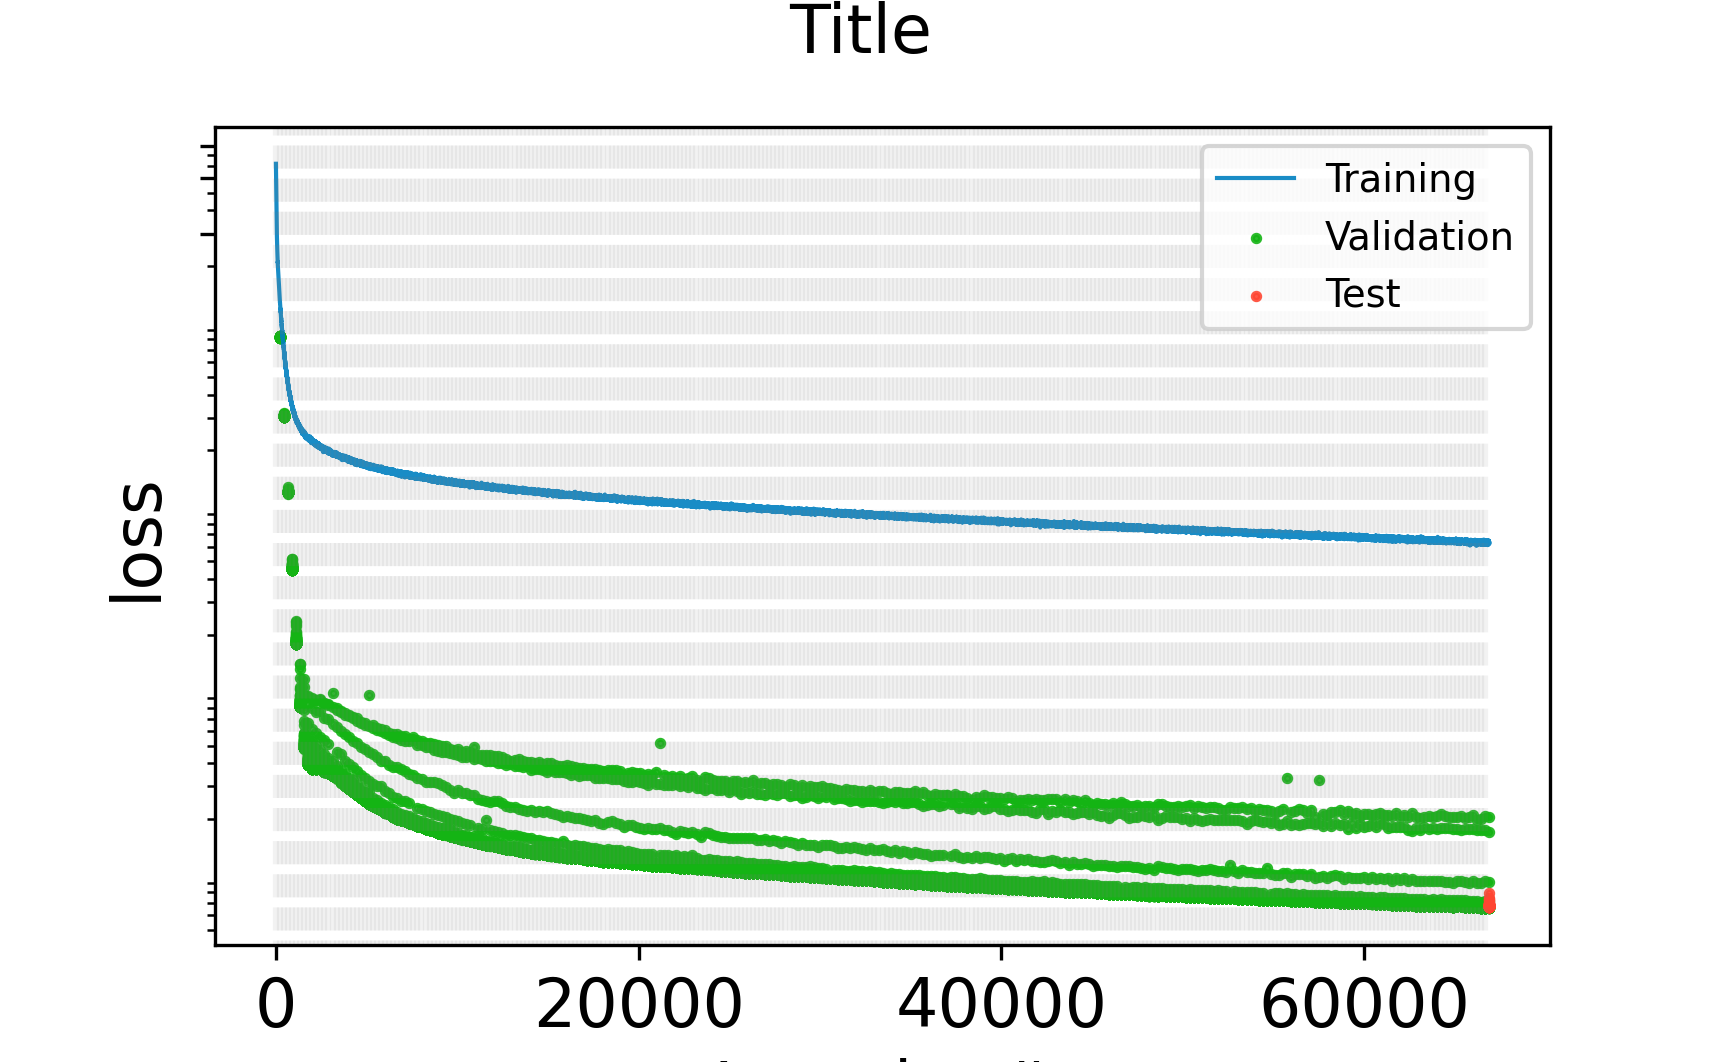
\includegraphics[width=1\textwidth]{./src/figures/1_3_png/Figure_ID_learning_curver_for_pretraining.png}
            \caption{\textbf{
Learning Curve of Pretraining
}
\smallskip
\\
\textbf{\textit{A.}} Figure Legend from Template.
}
% width=1\textwidth
            \label{fig:
learning_curver_for_pretraining}
        \end{figure*}

%%%%%%%%%%%%%%%%%%%%%%%%%%%%%%%%%%%%%%%%%%%%%%%%%%%%%%%%%%%%%%%%%%%%%%%%%%%%%%%%
%% END
%%%%%%%%%%%%%%%%%%%%%%%%%%%%%%%%%%%%%%%%%%%%%%%%%%%%%%%%%%%%%%%%%%%%%%%%%%%%%%%%

\end{document}
